\documentclass [a4paper, 11pt] {article}

\newcommand\seancetitle{Encodage}
\newcommand\seancenumber{3}
\def\AvecSolutions{}  % Commenter pour ne pas afficher les solutions

\usepackage[utf8]{inputenc}  
\usepackage[T1]{fontenc}  
\usepackage{lmodern}
\usepackage[french]{babel}
\usepackage{fancybox}
\usepackage{listings}
\usepackage{color}
\usepackage{tikz}
\usetikzlibrary{babel}
\usetikzlibrary{decorations.markings}
\usepackage{pgfplots}
\pgfplotsset{compat=1.18}
\pgfplotsset{samples=200}
\usepackage{graphicx,subfigure}
\usepackage[titletoc]{appendix}
\usepackage{float} % figures flottantes 
\usepackage{here} % figures flottantes
\usepackage{url}
\usepackage{enumitem}
\setlist[itemize]{label={$\bullet$}}
%\setlist[enumerate]{noitemsep, nolistsep}
\usepackage{xcolor}
\usepackage[colorlinks=true]{hyperref}
\usepackage{tabularx}
\usepackage{minted}
\usepackage{amsmath}
\usepackage[skins,breakable]{tcolorbox}
\usepackage{verbatim}
\usepackage[europeanresistors,siunitx]{circuitikz}
\usepackage{multicol}
\usepackage{physics}
\usepackage[outline]{contour} % glow around text
%\usetikzlibrary{intersections}
%\usetikzlibrary{decorations.markings}
\usetikzlibrary{angles,quotes} % for pic
\usetikzlibrary{bending} % for arrow head angle
\contourlength{1.0pt}
\usetikzlibrary{3d}
\usetikzlibrary{trees}
\usepackage{dirtytalk}

% --------------------------------------------------------------
% Title
% --------------------------------------------------------------
\makeatletter
\newcommand\maintitle[1]{
    \quitvmode
    \hb@xt@\linewidth{
        \dimen@=1ex
        \advance\dimen@-2pt
        \leaders\hrule \@height1ex \@depth-\dimen@\hfill
        \enskip
        \textbf{#1}
        \enskip
        \leaders\hrule \@height1ex \@depth-\dimen@\hfill
    }
}
\makeatother

\newcommand{\makeseancetitle}{
\begin{center}
    \Large
    \centering
    \maintitle{LELEC1930 - Introduction aux télécommunications}\\
    \textsc{\textbf{Séance \seancenumber{} - \seancetitle{}}}\\
    \vspace{0.1cm}
    \normalsize
    Prof. : Jérôme Louveaux \hfill Assist. : Jérome Eertmans\\
   \noindent\hrulefill
\end{center}
}

\newcommand{\makerappeltitle}{
\begin{center}
    \Large
    \centering
    \maintitle{LELEC1930 - Introduction aux télécommunications}\\
    \textsc{\textbf{Rappel - \seancetitle{}}}\\
    \vspace{0.1cm}
    \normalsize
    Prof. : Jérôme Louveaux \hfill Assist. : Jérome Eertmans\\
   \noindent\hrulefill
\end{center}
}

\usepackage{fancyhdr}
\fancypagestyle{firstpage}
{
   \cfoot{Page \thepage}
}
\fancypagestyle{nextpages}
{
    \lhead{Séance \seancenumber{}}
    \chead{\seancetitle}
    \rhead{LELEC1930}
    \cfoot{Page \thepage}
}
\fancypagestyle{rappelnextpages}
{
    \lhead{Rappel}
    \chead{\seancetitle}
    \rhead{LELEC1930}
    \cfoot{Page \thepage}
}

\setlength{\headheight}{13.59999pt}

% --------------------------------------------------------------
% Some parameters
% --------------------------------------------------------------
\oddsidemargin =0 mm
\topmargin = -10 mm
\footskip = 20mm
\textheight = 240 mm 
\textwidth = 160mm

% --------------------------------------------------------------
% Exercice environments
% --------------------------------------------------------------
\newcounter{exercice}

\definecolor{exercice_color}{RGB}{21,76,121}
\definecolor{exercice_color_fill}{RGB}{252,248,227}

\newcommand{\theexerciceref}{No reference}

\makeatletter
\newenvironment{exercice}[2][\texorpdfstring{\unskip}{}]
{
\refstepcounter{exercice}
\def\@currentlabel{{#2}}
\label{ref-exercice-\theexercice}
\addcontentsline{toc}{subsubsection}{{#2} #1}
\noindent
\flushleft
\begin{tikzpicture}
    \draw[very thick,exercice_color] (0,0) -- ++(0,+7.5pt)
    -- ++(\textwidth,0) node[midway,above] {\textbf{Exercice #2 : #1}}
    -- ++(0,-7.5pt);
\end{tikzpicture}
\vspace{-.3cm}
\begin{tcolorbox}[
    blanker,
    width=\textwidth,
    breakable]
}
{   \end{tcolorbox}
\vspace{-.4cm}
\flushleft
\begin{tikzpicture}
    \draw[very thick,exercice_color] (0,0) -- ++(0,-7.5pt)
    -- ++(\textwidth,0)
    -- ++(0,+7.5pt);
\end{tikzpicture}
}
\makeatother

\ifcsname AvecSolutions\endcsname
\newenvironment{reponse}
{
\noindent
\begin{tcolorbox}[
    colframe=exercice_color,
    colback=exercice_color_fill,
    coltitle=exercice_color_fill,  
    title=\centering\textbf{{\hypersetup{allcolors=white} Réponse à l'exercice \ref{ref-exercice-\theexercice} :}},
    breakable,
    width=\textwidth]
}
{   \end{tcolorbox}
}
\else
\newenvironment{reponse}{\comment}{\endcomment}
\fi


% --------------------------------------------------------------
% Code environments
% --------------------------------------------------------------
\usemintedstyle{borland}
\providecommand*{\listingautorefname}{Listing}

\newenvironment{python}
{\VerbatimEnvironment
\begin{minted}[
linenos,
% fontfamily=courier,
fontsize=\normalsize,
xleftmargin=21pt,
]{python}}
{\end{minted}}

\newcommand\py[1]{\mintinline{python}{#1}}

\newcommand\la[1]{\mintinline{latex}{#1}}

% Vertical line in matrices

\makeatletter
\renewcommand*\env@matrix[1][*\c@MaxMatrixCols c]{%
  \hskip -\arraycolsep
  \let\@ifnextchar\new@ifnextchar
  \array{#1}}
\makeatother

% Double underline
\def\doubleunderline#1{\underline{\underline{#1}}}


\begin{document}

    \makeseancetitle
    \thispagestyle{firstpage}
    
    \part*{Rappel}
    
    \paragraph{Attention :} \textit{dans les exercices suivants, les opérations sont effectuées modulo 2. Le résultat est soit 0, soit 1. On aura donc que $1 + 1 = 0$, $1+1+1 =1$, $1+1+1 +1 =0$, etc.}
    
    \subsection*{Code correcteur}
    
    Lors de la transmission d'un message, il n'est pas rare d'observer une déformation du message lors de son chemin. De ce fait, l'information reçue peut ne contenir que de manière partielle le message original.
    
    En anticipation à ce problème, le message est alors envoyé sous une forme encodée, souvent plus longue, afin d'augmenter le taux de réussite quant à la bonne réception du message. De manière générale, on utilise \textbf{un dictionnaire} permettant d'encoder un message de $k$ bits sur $n$ bits. On définit le \textbf{taux du code} comme étant alors $\frac{k}{n}$.
    
    \begin{figure}[H]
        \centering
        \begin{equation*}
            \begin{matrix}
                00 \rightarrow \\
                01 \rightarrow\\
                10 \rightarrow\\
                11 \rightarrow\\
            \end{matrix}
            \begin{bmatrix}[cccccc]
               1 & 0 &  1 &  0 &  1 &  0 \\
               1 & 1 &  1 &  1 &  1 &  1\\
               0 & 0 &  0 &  0 &  0 &  0\\
               0 & 1 &  0 &  1 &  0 &  1\\
            \end{bmatrix}
        \end{equation*}
        \caption{Dictionnaire d'encodage d'un message de 2 bits sur 6 bits.}
        \label{fig:encodage}
    \end{figure}
    
    \textbf{La distance minimale} d'un code, notée $d_{min}$, est la plus petite distance entre deux mots du dictionnaire. La distance entre deux mots, aussi appelée distance de Hamming, est le nombre de bits différents entre ces deux mots. Dans l'exemple de la \autoref{fig:encodage}, la distance minimale est de 3 bits.
    
    Un code dont la distance minimale vaut $d_{min}$ détecte $d_{min}-1$ erreurs et peut corriger $\lfloor\frac{d_{min}-1}{2} \rfloor$ erreurs, où $\lfloor \cdot \rfloor$ est l'arrondi vers le bas. Ceci définit la \textbf{capacité correctrice} d'un code.
    
    Le décodage d'un bloc reçu se fait en recherchant le mot le plus proche de ce dernier en termes de distance. Exemple pour la \autoref{fig:encodage} :
    \begin{equation}
        \begin{bmatrix}
            1 & 0 & 1 & 1 & 1 & 0
        \end{bmatrix}
        \longrightarrow
        \begin{bmatrix}
            1 & 0 & 1 & \color{red} 0 & 1 & 0
        \end{bmatrix}
        \longrightarrow 00
    \end{equation}
    
    Un \textbf{code de Hamming} est un code correcteur linéaire qui permet la détection d'une erreur si elle n'est présente que sur une lettre du message. Les codes linéaires peuvent être complètement représenté par une \textbf{matrice génératrice} $\doubleunderline{G}$ de taille $k \times n$. Cette matrice s'obtient en assemblant les mots de codes correspondant à la base canonique\footnote{1000, 0100, 0010 et 0001 dans le cas d'un mot d'information de 4 bits.}. À partir de n'importe quel mot d'information $\underline{i}$, on peut calculer son mot de code, $\underline{c}$, en effectuant le produit matriciel $\underline{c} = \underline{i} \; \doubleunderline{G}$.
    
    \pagebreak
    \pagestyle{nextpages}
    
    On définit alors la \textbf{matrice de contrôle} $H$. Cette dernière est plus complexe à calculer dans un cas général. Néanmoins, lorsque la matrice $\doubleunderline{G}$ a une structure particulière formée d'une sous-matrice identité (ici représentée en noir sur la \autoref{fig:generatrice_encodage_hamming_7_4}) accolée à une autre sous-matrice (ici représentée en \textcolor{blue}{bleu}), dans ce cas, la matrice de parité  peut s'obtenir en transposant la partie \textcolor{blue}{bleue} de la matrice $\doubleunderline{G}$ et en y ajoutant une sous-matrice identité à droite pour compléter une matrice de taille $(n-k) \times n$. C'est le cas notamment pour la matrice du code de Hamming (voir ci-dessous).
    
    Pour un bloc reçu $\underline{c}$, le vecteur syndrome est donné par $\underline{s} = \underline{c} \; \doubleunderline{H}^T$.  Il indique la présence ou non d'erreur(s) :  le vecteur nul indique l'absence d'erreurs.
    
    \begin{figure}[H]
        \centering
        \begin{equation*}
            \begin{matrix}
               0000 \rightarrow \\
               0001 \rightarrow \\
               0010 \rightarrow \\
               0011 \rightarrow \\
               0100 \rightarrow \\
               0101 \rightarrow \\
               0110 \rightarrow \\
               0111 \rightarrow \\
            \end{matrix}
            \begin{bmatrix}[ccccccc]
               0 & 0 & 0 & 0 & \color{blue} 0 & \color{blue} 0 & \color{blue} 0 \\
               0 & 0 & 0 & 1 & \color{blue} 1 & \color{blue} 1 & \color{blue} 0 \\
               0 & 0 & 1 & 0 & \color{blue} 0 & \color{blue} 1 & \color{blue} 1 \\
               0 & 0 & 1 & 1 & \color{blue} 1 & \color{blue} 0 & \color{blue} 1 \\
               0 & 1 & 0 & 0 & \color{blue} 1 & \color{blue} 0 & \color{blue} 1 \\
               0 & 1 & 0 & 1 & \color{blue} 0 & \color{blue} 1 & \color{blue} 1 \\
               0 & 1 & 1 & 0 & \color{blue} 1 & \color{blue} 1 & \color{blue} 0 \\
               0 & 1 & 1 & 1 & \color{blue} 0 & \color{blue} 0 & \color{blue} 0 \\
            \end{bmatrix}
            \hspace{.3cm}\&\hspace{.4cm}
            \begin{matrix}
               1000 \rightarrow \\
               1001 \rightarrow \\
               1010 \rightarrow \\
               1011 \rightarrow \\
               1100 \rightarrow \\
               1101 \rightarrow \\
               1110 \rightarrow \\
               1111 \rightarrow \\
            \end{matrix}
            \begin{bmatrix}[ccccccc]
               1 & 0 & 0 & 0 & \color{blue} 1 & \color{blue} 1 & \color{blue} 1 \\
               1 & 0 & 0 & 1 & \color{blue} 0 & \color{blue} 0 & \color{blue} 1 \\
               1 & 0 & 1 & 0 & \color{blue} 1 & \color{blue} 0 & \color{blue} 0 \\
               1 & 0 & 1 & 1 & \color{blue} 0 & \color{blue} 1 & \color{blue} 0 \\
               1 & 1 & 0 & 0 & \color{blue} 0 & \color{blue} 1 & \color{blue} 0 \\
               1 & 1 & 0 & 1 & \color{blue} 1 & \color{blue} 0 & \color{blue} 0 \\
               1 & 1 & 1 & 0 & \color{blue} 0 & \color{blue} 0 & \color{blue} 1 \\
               1 & 1 & 1 & 1 & \color{blue} 1 & \color{blue} 1 & \color{blue} 1 \\
            \end{bmatrix}
        \end{equation*}
        \caption{Dictionnaire du code de Hamming (7,4).}
        \label{fig:encodage_hamming_7_4}
    \end{figure}
    
    \begin{figure}[H]
        \centering
        \begin{equation*}
            \doubleunderline{G} =
            \begin{bmatrix}[ccccccc]
               1 & 0 & 0 & 0 & \color{blue} 1 & \color{blue} 1 & \color{blue} 1 \\
               0 & 1 & 0 & 0 & \color{blue} 1 & \color{blue} 0 & \color{blue} 1 \\
               0 & 0 & 1 & 0 & \color{blue} 0 & \color{blue} 1 & \color{blue} 1 \\
               0 & 0 & 0 & 1 & \color{blue} 1 & \color{blue} 1 & \color{blue} 0 \\
            \end{bmatrix}
            \hspace{.7cm}
            \doubleunderline{H} =
            \begin{bmatrix}[ccccccc]
               \color{blue} 1 & \color{blue} 1 & \color{blue} 0 & \color{blue} 1 & 1 & 0 & 0 \\
               \color{blue} 1 & \color{blue} 0 & \color{blue} 1 & \color{blue} 1 & 0 & 1 & 0 \\
               \color{blue} 1 & \color{blue} 1 & \color{blue} 1 & \color{blue} 0 & 0 & 0 & 1 \\
            \end{bmatrix}
        \end{equation*}
        \caption{Matrice génératrice et matrice de contrôle du code de Hamming (7,4).}
        \label{fig:generatrice_encodage_hamming_7_4}
    \end{figure}
    
    \subsection*{Compression des données}
    
    Souvent, on souhaite réduire la taille des messages envoyés afin qu'ils soient transmis plus rapidement ou prennent moins de place sur un espace de stockage. Pour ce faire, les données sont compressées en utilisant un algorithme de codage. C'est le cas des fichiers \py{.zip} ou encore du codage de Huffman. Ce dernier est décrit dans les slides du cours et un exemple détaillé est disponible sur la page \href{https://fr.wikipedia.org/wiki/Codage_de_Huffman#Principe}{Wikipédia}.
    
    Le code de Huffman se base sur une distribution connue des symboles afin de créer un code de compression. Le code de compression se présente sous forme d'un arbre où prendre une branche à gauche indique un 0 et une branche à droite un 1. Ci-dessous, l'arbre obtenu pour la phrase \say{this is an example of a huffman tree}, pour lequel le code final est : \{'e' : 000, 'a' : 010, ' ' : 111, ...\}.
    
    \begin{figure}[H]
        \centering
        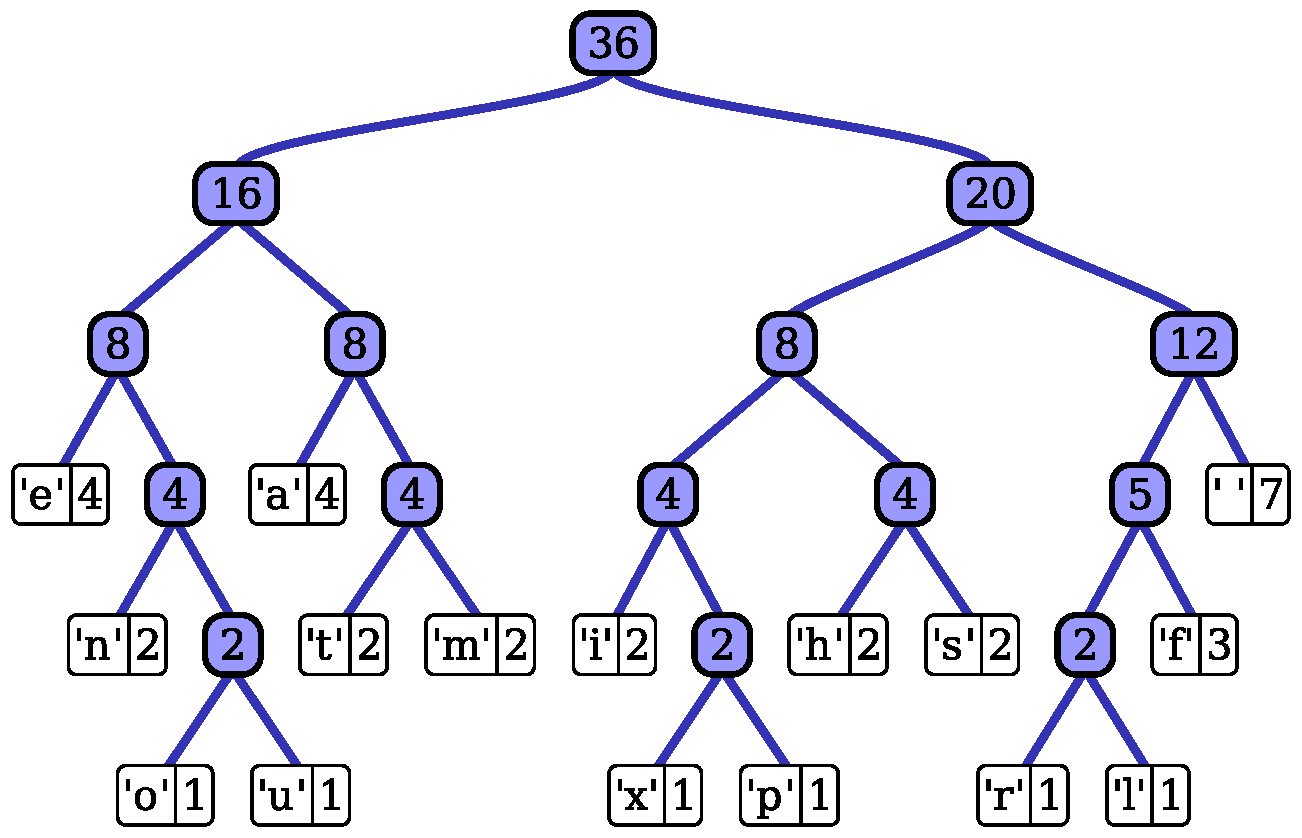
\includegraphics[width=.5\textwidth]{imgs/Huffman_tree_2.pdf}
        \caption{Arbre d'Huffman, repris de Wikipédia.}
        \label{fig:huffman}
        \vspace{-2cm}
    \end{figure}
    
    \pagebreak
    \pagestyle{nextpages}
    
    
    
    \pagebreak
    \part*{Exercices}
    
    \begin{exercice}[Dictionnaire d'un code]{1}
        
        À partir du code suivant :
        
        \begin{equation*}
            \begin{matrix}
                00 \rightarrow \\
                01 \rightarrow\\
                10 \rightarrow\\
                11 \rightarrow\\
            \end{matrix}
            \begin{bmatrix}[ccccccc]
               0 & 0 & 0 & 0 & 0 & 0 & 0 \\
               1 & 0 & 0 & 1 & 1 & 0 & 1\\
               0 & 1 & 1 & 0 & 1 & 0 & 1\\
               1 & 1 & 1 & 1 & 0 & 0 & 0\\
            \end{bmatrix}
        \end{equation*}
      
        \begin{enumerate}
            \item Calculez le taux du code.
            \item Effectuez le décodage du bloc reçu suivant : $y = \begin{bmatrix}
               1 & 0 & 1 & 1 & 1 & 1 & 1
            \end{bmatrix}$.
            \item Quelle est la capacité correctrice du code ?
            \item Il s'agit d'un code linéaire. Quelle est la taille de sa matrice de contrôle ?
        \end{enumerate} 
    \end{exercice}
    
    \begin{reponse}
        Le code présenté encode 2 bits ($k$) sur 7 bits ($n$).
        
        \begin{enumerate}
            \item Le taux est donc de $\frac{2}{7}$.
            \item Le code le plus proche de $y$ est $\begin{bmatrix}
               1 & 0 & \color{red} 0 & 1 & 1 & \color{red} 0 & 1
            \end{bmatrix}$, ce qui correspond au mot 01.
            \item On calcule que la distance minimale est de 4. La capacité correctrice est donc de 1. C'est le nombre minimum d'erreurs que l'on peut corriger : pas maximum. Sinon, on n'aurait pas pu corriger $y$.
        \end{enumerate}
    \end{reponse}
    
    \begin{exercice}[Code de Hamming]{2}
        
        Considérez le code de Hamming (7,4) et répondez aux questions suivantes :
      
        \begin{enumerate}
            \item Calculez le mot codé pour les bits d'entrée 1101.
            \item Quel est le taux de ce code ?
            \item Quelle est la distance minimale du code ?
            \item Calculez le syndrome du code 1111110.
            \item Quel est le mot à l'origine du code 1001101 ?
            \item Quel est le mot à l'origine du code 0000110 ?
        \end{enumerate} 
    \end{exercice}
    
    \begin{reponse}
        Pour répondre aux questions, il est utile de relire le rappel.
        \begin{enumerate}
            \item 1101 devient 1101100.
            \item Le taux est de $\frac{4}{7}$.
            \item La distance minimale est de 3.
            \item Le syndrome de $\underline{c}=1111110$ est $\underline{s} = \underline{c} \times \doubleunderline{H}^T=001$.
            \item Le mot le plus proche est 1001.
            \item Le mot le plus proche est 0001.
        \end{enumerate}
    \end{reponse}
    
    \begin{exercice}[Code de Huffman]{3}
      
        \begin{enumerate}
            \item Parmi les codes suivants, lesquels \textbf{ne sont pas} des codes de Huffman ?
            \begin{enumerate}
                \item \{1, 01, 00\}
                \item \{01, 11, 10\}
                \item \{00, 01, 10, 110\}
                \item \{0, 1, 01, 11\}
            \end{enumerate}
            \item On considère une source d’information, ayant 5 valeurs possibles, avec les probabilités données ci-dessous. On considère aussi deux encodages possibles $C_1$ et $C_2$ :
            \begin{center}
            \begin{tabular}{c|c|ll}
                 $x$ & $p(x)$ & $C_1$ & $C_2$ \\
                 \hline
                 a & 0.50 & 0 & 01\\
                 b & 0.15 & 10 & 00\\
                 c & 0.15 & 110 & 10\\
                 d & 0.10 & 1110 & 110\\
                 e & 0.10 & 1111 & 111\\
            \end{tabular}
            \end{center}
            Quel code fournit la meilleure compression d'information ?
            \item Construisez l'arbre de Huffman pour la phrase \say{Ésope reste ici et se repose}.
        \end{enumerate} 
    \end{exercice}
    
    \begin{reponse}
        \begin{enumerate}
            \item Pour vérifier si un code est valide, il faut tracer un arbre et vérifier que chaque feuille possède une paire. Par exemple, si le code 01 existe, alors le code 00 ou ses deux feuilles doivent exister. Une feuille (un code) ne peut pas posséder de sous-feuille.
            \begin{enumerate}
                \item Code de Huffman.
                \item Non valide, car 01 n'a pas sa paire.
                \item Non valide, car 110 n'a pas sa paire.
                \item Non valide, car 0 et 1 sont des feuilles et ne peuvent donc pas avoir de sous-feuille.
            \end{enumerate}
            \item Pour estimer la compression de chaque code, on peut calculer le nombre de bits moyen et comparer :
            \begin{align*}
                \overline{C}_1 &= 0.50 \cdot 1 + 0.15 \cdot 2 + 0.15 \cdot 3 + 0.10 \cdot 4 + 0.10 \cdot 4 = 2.05\\
                \overline{C}_2 &= 0.50 \cdot 2 + 0.15 \cdot 2 + 0.15 \cdot 2 + 0.10 \cdot 3 + 0.10 \cdot 3 = 2.20
            \end{align*}
            Le premier code est donc légèrement meilleur.
            \item Voici un exemple d'arbre que vous pouvez obtenir. Des variations sont possibles, car plusieurs lettres apparaissent le même nombre de fois.
            \begin{center}
                \begin{tikzpicture}[iv/.style={draw,fill=red!50,circle,minimum size=20pt,inner sep=0pt,text=black},ev/.style={draw,fill=yellow,rectangle,minimum size=20pt,inner sep=2pt,text=black}]
                \node[iv]{28}
                  child {
                    node[iv]{12}
                    child {
                        node[ev]{espace(5)}
                        }
                    child [missing]
                    child {
                        node[iv]{7}
                        child {
                            node[iv]{3}
                            child {
                                node[ev]{C(1)}
                            }
                            child {
                                node[ev]{O(2)}
                            }
                        }
                        child [missing]
                        child {
                            node[iv]{4}
                            child {
                                node[ev]{T(2)}
                            }
                            child {
                                node[ev]{I(2)}
                            }
                        }
                    }
                    edge from parent node[above]{0}        
                }
                child [missing]
                child [missing]
                child [missing]
                child [missing]
                child {
                    node[iv]{16}
                    child {
                        node[iv]{8}
                        child {
                            node[iv]{4}
                            child {
                                node[ev]{P(2)}
                            }
                            child {
                                node[ev]{R(2)}
                            }
                        }
                        child {
                            node[ev]{S(4)}
                        }
                    }
                    child {
                        node[ev]{E(8)}
                        }
                    edge from parent node[above]{1}        
                };
                \end{tikzpicture}
            \end{center}
        \end{enumerate}
    \end{reponse}
    
    \begin{exercice}[Planning de fréquence]{4 (bonus)}
        On veut établir le planning de fréquence d’un réseau cellulaire. En raison de différents effets de propagation, on suppose que la densité de puissance reçue à une distance $r$ ($r >\SI{10}{\meter}$) d’une station de base est approximée par
        \begin{equation}
            S(r) = \frac{P_0}{r^3},
        \end{equation}
        où $P_0$ est la puissance de l’antenne (supposée identique pour toutes les stations de base). Pour simplifier, on suppose que toutes les cellules sont des cercles de \SI{1}{\kilo\meter} de rayon centrés sur leur station de base respective. Quelle doit être la distance minimale entre 2 stations de base réutilisant la même fréquence, de façon à ce que signal utile en provenance de la première station de base soit toujours au minimum \SI{20}{\decibel} au-dessus de l’interférence en provenance de la deuxième station de base ?
    \end{exercice}
    
    \begin{reponse}
        Afin de répondre à l'exercice, il est utile de faire un petit dessin, voir la \autoref{fig:planning}. L'utilisateur (en \textcolor{red}{rouge}), souhaite donc recevoir un signal de la part de $TX_1$ au minimum \SI{20}{\decibel} au-dessus de $TX_2$.
        
        Le pire cas de figure est celui illustré : l'utilisateur est en bordure de zone ($d_1=\SI{1}{\kilo\meter}$) et se trouve au plus proche de $TX_2$.
        \begin{figure}[H]
            \centering
            \begin{tikzpicture}
                \pgfmathsetmacro{\onekm}{2}
                \coordinate (A1) at (0,0);
                \filldraw [very thick,draw=black,dashed,fill=gray!20] (A1) circle (\onekm);
                \node[circle,draw,fill,label=above:{$TX_1$}] (N1) at (A1) {};
                \path (A1) -- ++(2.5*\onekm,0) coordinate (A2);
                \filldraw [very thick,draw=black,dashed,fill=gray!20] (A2) circle (\onekm);
                \node[circle,draw,fill,label=above:{$TX_2$}] (N2) at (A2) {};
                \path (A1) ++ (\onekm,0) node[circle,draw=black,fill=red] (U) {};
                \draw[|<->|,dashed] (N1) -- (U) node[midway,above] {$d_1$};
                \draw[|<->|,dashed] (U) -- (N2) node[midway,above] {$d_2$};
            \end{tikzpicture}
            \caption{Schéma du problème.}
            \label{fig:planning}
        \end{figure}
        
        La distance $d_1=1$ km. On veut aussi que le rapport des puissances soit de \SI{20}{\decibel}, c.-à-d. un rapport de 100 :
        \begin{equation}
            \frac{S_1}{S_2} = 100 = \frac{d_2^3}{d_1^3} \Rightarrow d_2 = \SI{4.64}{\kilo\meter}.
        \end{equation}
        La distance entre les deux antennes doit donc être de \SI{5.64}{\kilo\meter}.
        
    \end{reponse}

\end{document}